%%%%%%%%%%%%%%%%%%%%%%%%%%%%%%%%%%%%%%%%%
% Article EcoFoG
% Version 2.1 (23/10/2017)
%
% adapté de :
% Stylish Article
% LaTeX Template
% Version 1.0 (31/1/13)
%
% This template has been downloaded from:
% http://www.LaTeXTemplates.com
%
% Original author:
% Mathias Legrand (legrand.mathias@gmail.com)
%
% License:
% CC BY-NC-SA 3.0 (http://creativecommons.org/licenses/by-nc-sa/3.0/)
%
%%%%%%%%%%%%%%%%%%%%%%%%%%%%%%%%%%%%%%%%%


%----------------------------------------------------------------------------------------
%	PACKAGES AND OTHER DOCUMENT CONFIGURATIONS
%----------------------------------------------------------------------------------------

\documentclass[fleqn,10pt]{ArtEcoFoG} % Document font size and equations flushed left

\setcounter{tocdepth}{3} % Show only three levels in the table of contents section: sections, subsections and subsubsections


% Pandoc environments
\usepackage{framed}
\usepackage{fancyvrb}
\providecommand{\tightlist}{%
  \setlength{\itemsep}{0pt}\setlength{\parskip}{0pt}}
\newcommand{\VerbBar}{|}
\newcommand{\VERB}{\Verb[commandchars=\\\{\}]}
\DefineVerbatimEnvironment{Highlighting}{Verbatim}{commandchars=\\\{\}, fontsize=\scriptsize} % Code R
\definecolor{shadecolor}{RGB}{248,248,248}
\newenvironment{Shaded}{\begin{snugshade}}{\end{snugshade}}
\newcommand{\KeywordTok}[1]{\textcolor[rgb]{0.13,0.29,0.53}{\textbf{{#1}}}}
\newcommand{\DataTypeTok}[1]{\textcolor[rgb]{0.13,0.29,0.53}{{#1}}}
\newcommand{\DecValTok}[1]{\textcolor[rgb]{0.00,0.00,0.81}{{#1}}}
\newcommand{\BaseNTok}[1]{\textcolor[rgb]{0.00,0.00,0.81}{{#1}}}
\newcommand{\FloatTok}[1]{\textcolor[rgb]{0.00,0.00,0.81}{{#1}}}
\newcommand{\ConstantTok}[1]{\textcolor[rgb]{0.00,0.00,0.00}{{#1}}}
\newcommand{\CharTok}[1]{\textcolor[rgb]{0.31,0.60,0.02}{{#1}}}
\newcommand{\SpecialCharTok}[1]{\textcolor[rgb]{0.00,0.00,0.00}{{#1}}}
\newcommand{\StringTok}[1]{\textcolor[rgb]{0.31,0.60,0.02}{{#1}}}
\newcommand{\VerbatimStringTok}[1]{\textcolor[rgb]{0.31,0.60,0.02}{{#1}}}
\newcommand{\SpecialStringTok}[1]{\textcolor[rgb]{0.31,0.60,0.02}{{#1}}}
\newcommand{\ImportTok}[1]{{#1}}
\newcommand{\CommentTok}[1]{\textcolor[rgb]{0.56,0.35,0.01}{\textit{{#1}}}}
\newcommand{\DocumentationTok}[1]{\textcolor[rgb]{0.56,0.35,0.01}{\textbf{\textit{{#1}}}}}
\newcommand{\AnnotationTok}[1]{\textcolor[rgb]{0.56,0.35,0.01}{\textbf{\textit{{#1}}}}}
\newcommand{\CommentVarTok}[1]{\textcolor[rgb]{0.56,0.35,0.01}{\textbf{\textit{{#1}}}}}
\newcommand{\OtherTok}[1]{\textcolor[rgb]{0.56,0.35,0.01}{{#1}}}
\newcommand{\FunctionTok}[1]{\textcolor[rgb]{0.00,0.00,0.00}{{#1}}}
\newcommand{\VariableTok}[1]{\textcolor[rgb]{0.00,0.00,0.00}{{#1}}}
\newcommand{\ControlFlowTok}[1]{\textcolor[rgb]{0.13,0.29,0.53}{\textbf{{#1}}}}
\newcommand{\OperatorTok}[1]{\textcolor[rgb]{0.81,0.36,0.00}{\textbf{{#1}}}}
\newcommand{\BuiltInTok}[1]{{#1}}
\newcommand{\ExtensionTok}[1]{{#1}}
\newcommand{\PreprocessorTok}[1]{\textcolor[rgb]{0.56,0.35,0.01}{\textit{{#1}}}}
\newcommand{\AttributeTok}[1]{\textcolor[rgb]{0.77,0.63,0.00}{{#1}}}
\newcommand{\RegionMarkerTok}[1]{{#1}}
\newcommand{\InformationTok}[1]{\textcolor[rgb]{0.56,0.35,0.01}{\textbf{\textit{{#1}}}}}
\newcommand{\WarningTok}[1]{\textcolor[rgb]{0.56,0.35,0.01}{\textbf{\textit{{#1}}}}}
\newcommand{\AlertTok}[1]{\textcolor[rgb]{0.94,0.16,0.16}{{#1}}}
\newcommand{\ErrorTok}[1]{\textcolor[rgb]{0.64,0.00,0.00}{\textbf{{#1}}}}
\newcommand{\NormalTok}[1]{{#1}}
\usepackage{longtable,booktabs}
\usepackage{caption}
% These lines are needed to make table captions work with longtable:
\makeatletter
\def\fnum@table{\tablename~\thetable}
\makeatother
% longtable 2 columns
% https://tex.stackexchange.com/questions/161431/how-to-solve-longtable-is-not-in-1-column-mode-error
\makeatletter
\let\oldlt\longtable
\let\endoldlt\endlongtable
\def\longtable{\@ifnextchar[\longtable@i \longtable@ii}
\def\longtable@i[#1]{\begin{figure}[t]
\onecolumn
\begin{minipage}{0.5\textwidth}\scriptsize
\oldlt[#1]
}
\def\longtable@ii{\begin{figure}[t]
\onecolumn
\begin{minipage}{0.5\textwidth}\scriptsize
\oldlt
}
\def\endlongtable{\endoldlt
\end{minipage}
\twocolumn
\end{figure}}
\makeatother

\usepackage{graphicx,grffile}
\makeatletter
\def\maxwidth{\ifdim\Gin@nat@width>\linewidth\linewidth\else\Gin@nat@width\fi}
\def\maxheight{\ifdim\Gin@nat@height>\textheight0.8\textheight\else\Gin@nat@height\fi}
\makeatother
% Scale images if necessary, so that they will not overflow the page
% margins by default, and it is still possible to overwrite the defaults
% using explicit options in \includegraphics[width, height, ...]{}
\setkeys{Gin}{width=\maxwidth,height=\maxheight,keepaspectratio}

% User-adder preamble
\usepackage{textcomp} \DeclareUnicodeCharacter{B0}{\textdegree}
\hyphenation{sa-plings} \usepackage{longtable,tabu}

%----------------------------------------------------------------------------------------
%	ARTICLE INFORMATION
%----------------------------------------------------------------------------------------

\JournalInfo{Hal xxx} % Journal information
\Archive{DOI xxxx} % Additional notes (e.g. copyright, DOI, review/research article)

\PaperTitle{Post-Disturbance Tree Community Trajectories in a Neotropical Forest} % Article title

\Authors{
Ariane MIRABEL\textsuperscript{1*}\\ Eric Marcon\textsuperscript{1}\\ Bruno Hérault\textsuperscript{2 3}
} % Authors
\affiliation{
\textsuperscript{1}UMR EcoFoG, AgroParistech, CNRS, Cirad, INRA, Université des Antilles,
Université de Guyane.\\ \hspace{1em} Campus Agronomique, 97310 Kourou, France.\\\textsuperscript{2}Cirad, Univ montpellier, UR Forests \& Societies.\\ \hspace{1em} Montpellier, France.\\\textsuperscript{3}INPHB, Institut National Polytechnique Félix Houphouet-Boigny\\ \hspace{1em} Yamoussoukro, Ivory Coast.
}
\affiliation{*\textbf{Corresponding author}: ariane.mirabel@ecofog.gf, http://www.ecofog.gf/spip.php?article47} % Corresponding author

\Keywords{mot-clés, séparés par des virgules} % Keywords - if you don't want any simply remove all the text between the curly brackets
\newcommand{\keywordname}{Keywords} % Defines the keywords heading name

%----------------------------------------------------------------------------------------
%	ABSTRACT
%----------------------------------------------------------------------------------------

\Abstract{
Résumé de l'article.
}

%----------------------------------------------------------------------------------------

\usepackage{amsthm}
\newtheorem{theorem}{Theorem}[section]
\newtheorem{lemma}{Lemma}[section]
\theoremstyle{definition}
\newtheorem{definition}{Definition}[section]
\newtheorem{corollary}{Corollary}[section]
\newtheorem{proposition}{Proposition}[section]
\theoremstyle{definition}
\newtheorem{example}{Example}[section]
\theoremstyle{definition}
\newtheorem{exercise}{Exercise}[section]
\theoremstyle{remark}
\newtheorem*{remark}{Remark}
\newtheorem*{solution}{Solution}
\begin{document}

\selectlanguage{english}

\flushbottom % Makes all text pages the same height

\maketitle % Print the title and abstract box

\tableofcontents % Print the contents section

\thispagestyle{empty} % Removes page numbering from the first page

%----------------------------------------------------------------------------------------
%	ARTICLE CONTENTS
%----------------------------------------------------------------------------------------


\begin{verbatim}
## Warning: package 'kableExtra' was built under R version 3.3.3
\end{verbatim}

\begin{verbatim}
## Warning: package 'shape' was built under R version 3.3.3
\end{verbatim}

\section{Introduction}\label{introduction}

The large areas covered with tropical forests worldwide hold crucial
economic, social and cultural value. They provide wood and multiple
non-timber forest products, shelter a diversified fauna, regulate local
climate, support carbon, water and nutrient cycles, and ensure cultural
and human well-being. The simultaneous increase of forests products
demand and substantial climatic changes heightened the pressure on the
remaining forests \citep{Gibson2011a, Morales-Hidalgo2015} and threaten
the maintenance of communities structure, composition and functioning
and the dynamics that shape them
\citep{Anderson-Teixeira2013, Sist2015}.

In tropical forests, a constant range of disturbance determines the
ecological rules shaping the communities through the reallocation of
resources (as light, heat and water fluxes), changes in interspecific
relations, etc. The response of communities to disturbance is then the
cornerstone of tropical forests ecology, modelling and management
\citep{White2001, Chazdon2003a}. Disturbance recovery have been largely
studied through structural parameters as aboveground biomass, tree
height or stem density, which all reflect rapid and measurable changes
of ecosystems functioning asses crucial issues about the maintenance of
ecosystems processes and services
\citep{Denslow2000, Blanc2009, Rutishauser2016}. In this perspective
tree species diversity is inevitable as it determines ecosystems
productivity, stability and functioning through the interspecific
complementarity that enhances resources use, nutrients storing, and
hazards mitigation \citep{Tilman2014}. Revealing diversity dynamics is
besides all the more important that disturbance, modifies the
environment and interspecific relations and surely impacts trees
composition and diversity \citep{CazzollaGatti2014}.

Until now, although, short-term dynamics demonstrated negligible or even
positive impacts on communities diversity in accordance with the
intermediate disturbance hypothesis (IDH)
\citep{Molino2001, Kariuki2006a, Berry2008a}. The long-term response of
communities composition and diversity to disturbance remains unclear.
The IDH predicting a maximized species diversity at intermediate level
of disturbance has besides mainly been tested through species richness,
which gives limited or misleading information on forests recovery and
functioning \citep{Martin2015, Chaudhary2016}. Studies of communities
response to disturbance should encompass taxonomic composition and
evenness, which only can assess some conservation issues and the
ecological rules that determine communities abundance distribution
\citep{Magurran1988, Lavorel2002, Bellwood2006}. Beyond taxonomic
metrics, communities recovery should also encompass functional diversity
metrics \citep{Moretti2009, Baraloto2012a} through functional traits,
that are species biological attributes relating to individuals fitness
and ecosystem properties \citep{Violle2007b, Scheiter2013}. Functional
traits were largely adopted and integrated within a workable framework
to assess forests dynamics and functioning
\citep{Diaz2005, Villeger2008a} and a vast litterature revealed some
major functional traits determinant for species ecology and performance.
These major traits proved relevant to assess the ecological rules
shaping species assembly: post-disturbance trajectories in tropical
rainforests, for example, are assumed to be driven by environmental
filters fostering disturbance resistant species with rapid growth and
efficient resources acquisition \citep{Molino2001, Haddad2008}.
Communities dynamics would then be reflected by a shift from
``conservative'' species displaying long-lived, dense tissues growing
slowly but with scarce resources, to ``acquisitive'' species with
fast-growing, light tissues allowing fast resources acquisition
\citep{TerSteege2001, Reich2014, Herault2011}. In this perspective a
combination of resource acquisition traits (leaf area, density and
chlorophyll content and stem specific gravity and bark thickness) and
life history traits of growth and reproduction (seed mass and maximum
height) already proved relevant
\citep{Wright2004, Westoby2006a, Chave2009b}.

Here we investigated over 30 years the response of 75 ha of forests
plots set up on a gradient of disturbance intensity, from 10 to 60\% of
ecosystem biomass removed. We made use of a large functional traits
database browsing major leaf, stem and seed traits and species maximum
height to draw communities taxonomic and functional composition and
diversity trajectories after disturbance. Specifically, we (i) tested
the validity of the IDH arguing for enhanced diversity after moderate
disturbance and (ii) confirmed the changes in ecological rules shaping
communities, from competitive exclusion between ``conservative'',
slow-growing tree species to environmental filtering of ``acquisitive'',
fasting-growing ones. Eventually we examined the different trajectories
to (iii) resolve the resilience of tropical forests and question their
future dynamics regarding their state 30 years after disturbance.

\section{Material and Methods}\label{material-and-methods}

\subsection{Study site}\label{study-site}

Paracou station in French Guiana (5°18'N and 52°53'W) is located in a
lowland tropical rain forest corresponding to a tropical wet climate
with mean annual precipitation averaging 2980 mm.y\textsuperscript{-1}
(30-y period) with a 3-months dry season (\textless{} 100
mm.months\textsuperscript{-1}) from mid-August to mid-November, and a
one-month dry season in March \citep{Wagner2011}. Elevation ranges
between 5 and 50 m and mean annual temperature is 26°C. Soils correspond
to thin acrisols over a layer of transformed saprolite with low
permeability generating lateral drainage during heavy rains. The
experiment corresponds to a network of twelve 6.25ha plots that have
undergone a gradient of three logging, thinning and fuelwood treatments
(Table \ref{tab:Tab1}). Disturbance treatments were attributed according
to a randomized plot design with three replicate blocks of four plots.
The disturbance corresponds to averages of 10 trees removed per hectare
with a diameter at 1.3 m height (DBH) above 50 cm for treatment 1 (T1),
32 trees/ha above 40 cm DBH for treatment 2 (T2) and 40 trees above 40
cm DBH for treatment 3 (T3). Treatments T2 and T3 besides included the
thinning of trees by poison girdling \citep{Blanc2009}.

\begin{longtabu} to \linewidth {>{\raggedright}X>{\raggedright}X>{\raggedright}X>{\raggedright}X>{\raggedright}X}
\caption{\label{tab:Tab1}Intervention table, summary of the disturbance intensity for the 4 plot treatments in Paracou.}\\
\toprule
Treatment & Timber & Thinning & Fuelwood & \%AGB lost\\
\midrule
Control &  &  &  & 0\\
T1 & DBH $\geq$ 50 cm, commercial species, ~ 10 trees/ha &  &  & $[12\%-33\%]$\\
T2 & DBH $\geq$ 50 cm, commercial species, ~ 10 trees/ha & DBH $\geq$ 40 cm, non-valuable species, ~ 30 trees/ha &  & $[33\%-56\%]$\\
T3 & DBH $\geq$ 50 cm, commercial species, ~ 10 trees/ha & DBH $\geq$ 50 cm, non-valuable species, ~ 15 trees/ha & 40 cm $\leq$ DBH $\leq$ 50 cm, non-valuable species, ~ 15 trees/ha & $[35\%-56\%]$\\
\bottomrule
\end{longtabu}

\subsection{Inventories protocol and dataset
collection}\label{inventories-protocol-and-dataset-collection}

The study site corresponds to a tropical rainforest with a dominance of
Fabaceae, Chrysobalanaceae, Lecythidaceae and Sapotaceae botanical
families. In the twelve experimental plots of the experiment, all trees
above 10 cm DBH were mapped and measured annually since 1984. During
inventories, trees were first identified with a vernacular name assigned
by the field team, and afterward with a scientific name assigned by a
botanist during regular botanical campaigns. In 1984, specific
vernacular names were given to 62 commercial or common species whereas
other less common species were identified under two identifiers only
separating trees and palm trees. The botanical campaigns carried every 5
to 6 years to identify all trees at the species level only started in
2003 and identification practices varied among plots and successive
campaigns. This raised methodological issues as vernacular names usually
correspond to different botanical species, resulting in significant
taxonomic uncertainties that had to be propagated to composition and
diversity metrics throught a Bayesian framework. The uncertainty
propagation was done by the replenishment of inventories completed at
genus level from real incomplete ones on the basisof
vernacular/botanical names association.

Vernacular names were replaced through multinomial trials
\(M_v\Big(\big[s_1, s_2, …, s_N\big],\big[\alpha_1, \alpha_2,…, \alpha_3\big]\Big)\)
based on the observed association probability
\(\big[\alpha_1, \alpha_2,…, \alpha_3\big]\) between each vernacular
name \emph{v} and the species \(\big[s_1, s_2, …, s_N\big]\) recorded in
the inventory.

To avoid remaining identification caveats and consider complete
inventories, the simulated inventories were then reported at genus. See
appendix 1 and \citet{Aubry-Kientz2013} for the detailed methodology.

The functional diversity metrics used a dataset for 6 functional traits
representing leaf economics (leaves thickness, toughness, total
chlorophyll content and specific leaf area, the leaf area per unit dry
mass) and wood economics (wood specific gravity and bark thickness), and
life history traits (maximum specific height and seed mass).

The trait database came from the BRIDGE project {[}\^{}1{]} where traits
values were assessed from a selection of individuals located in nine
permanent plots in French Guiana, including two in Paracou. Missing
trait values were filled using multivariate imputation by chained
equation (mice) restricted to samples pertaining to the next higher
taxonomic level, in order to account for the phylogenetic signal of the
functional traits. The dataset comprised 294 botanical species
pertaining to 157 botanical genera.

Whenever a species inventoried was not in the dataset, it was attributed
a set of traits values randomly sampled among species of the same next
higher taxonomic level. As seed mass information corresponds to a
classification into mass classes, no data filling process was applied so
analysis were performed considering the 414 botanical species of the
seed mass dataset. All composition and diversity metrics corresponded to
the average obtained after 50 iterations of the taxonomic uncertainty
propagation framework and of the filling process of missing trait
values.

{[}\^{}1{]} http://www.ecofog.gf/Bridge/

\subsection{Composition and diversity
metrics}\label{composition-and-diversity-metrics}

To counter the remaining taxonomic uncertainty plots taxonomic
composition and diversity were analysed at the genus level, \emph{i.e.}
referring to the genus of observed or trialed botanical names. The
analysis of taxonomic and functional composition of plots along time was
visualized in a two-dimensional ordination space based on non-metric
dimensional scaling of succesive floristic or functional inventories.
Plots trajectories along time was reported comparatively to the
inventories in 1989, 5 years after disturbance, which corresponded to
first inventory with a sufficient degree of uncertainty (\textless{}30\%
of undetermined trees). The inventories dissimilarity compared to the
reference 1989 inventory was reported using occurrence-based (Jaccard)
and abundance-based (Bray-Curtis) similarity measures. The trajectory of
inventories along time was visualized with the euclidean distance in the
two-dimensional ordination space to the 1989 inventory. The functional
trajectories of the leaf and stem and life traits were also visualized
with the community weighted means (CWM), representing the average trait
value in a community weighted by relative abundance of the species
carrying each value \citep{Diaz2007, Garnier2004}. Species seed mass
correspond to 5 classes of increasing mass, the seed mass trajectories
were reported by the proportion of each class recorded in the
inventories. To determine whether communities' assembly deviated from
the expectation of a random process we compared the observed similarity
patterns to those generated by 50 repetitions of stochastic null models.
The null model for taxonomic composition randomly shuffled individuals
among plots while preserving the overall species abundance and plots'
tree density. The null model for functional composition produced random
traits assemblages by permuting the set of functional traits values
among species.

The taxonomic diversity was assessed through Richness and the Hill
number translation of Shannon and Simpson indices \citep{Hill1973}. To
tackle the unequal number of recruited trees among treatments the
indices bias corrected estimator were used, following
\citep{Chao2015, Marcon2015b}. These three indices belong to the set of
HCDT or generalized entropy, respectively corresponding to the 0, 1 and
2 order of diversity (q), which proved well suited for diversity studies
\citep{Patil1982, Tothmeresz1995}. The functional diversity was reported
using the Rao index of quadratic entropy which combines species
abundance distribution and average pairwise dissimilarity based on all
functional and life traits.

\section{Results}\label{results}

\subsection{Taxonomic and functional
composition}\label{taxonomic-and-functional-composition}

\subsubsection{Composition trajectories}\label{composition-trajectories}

Over time, 828388 trees and 591 botanical species pertaining to 223
genus and 64 botanical families were recorded. Trajectories of taxonomic
and functional composition after disturbance were examined through the
ordination of successive inventories from 1989 (5 years after
disturbance) in the two-dimensional space from NMDS analysis based on
flora inventories and the corresponding functional composition.
Classifications were performed using either abundance-based Bray-Curtis
(Figure \ref{fig:Fig1}) or incidence-based Jaccard dissimilarity (data
not shown).

Both taxonomic and functional composition were substantially affected by
disturbance, and the maximum dissimilarity to 1984 reference inventory
composition was positively correlated with the disturbance intensity.
Until 30 years after disturbance, all disturbed plots taxonomic
composition remained significantly dissimilar to that of the 1989
reference inventory composition (Figure \ref{fig:Fig1}). All plots,
though, displayed a unimodal trajectory with a the return toward the
taxonomic and functional composition of the 1989 reference inventory
suggesting a shift towards a cyclic regime (Figure \ref{fig:Fig2}). For
taxonomic composition, the maximum dissimilarity to 1984 inventory
composition was reach around 20 years after disturbance for the T2 and
T3 plots and for one T1 plot while control and other T1 plots continued
to increase (Figure \ref{fig:Fig2}.a). For functional composition, the
maximum dissimilarity to 1984 inventory composition was reach from 15 to
20 years after disturbance for the T2 and T3 plots while T1 and control
plots continued to increase (Figure \ref{fig:Fig2}.b). The functional
composition distancing from the reference inventory was also positively
correlated with disturbance intensity and similarly stabilized or
reduced (for 5 of T1, T2 and T3 plots) from 20 years after disturbance
(Figure \ref{fig:Fig2}).

\begin{quote}
The distance from the initial condition was significantly time-dependent
(P\textless{}0.01). The coordinates of the functional traits were
measured in the two-dimensional ordination space that mapped plots
evolution along time (graphs not showed) which revealed that the
trajectories of disturbed plots along time headed toward acquisitive
functional strategies (from high SWG to high SLA and chlorophyll
content).
\end{quote}

\begin{figure*}

{\centering 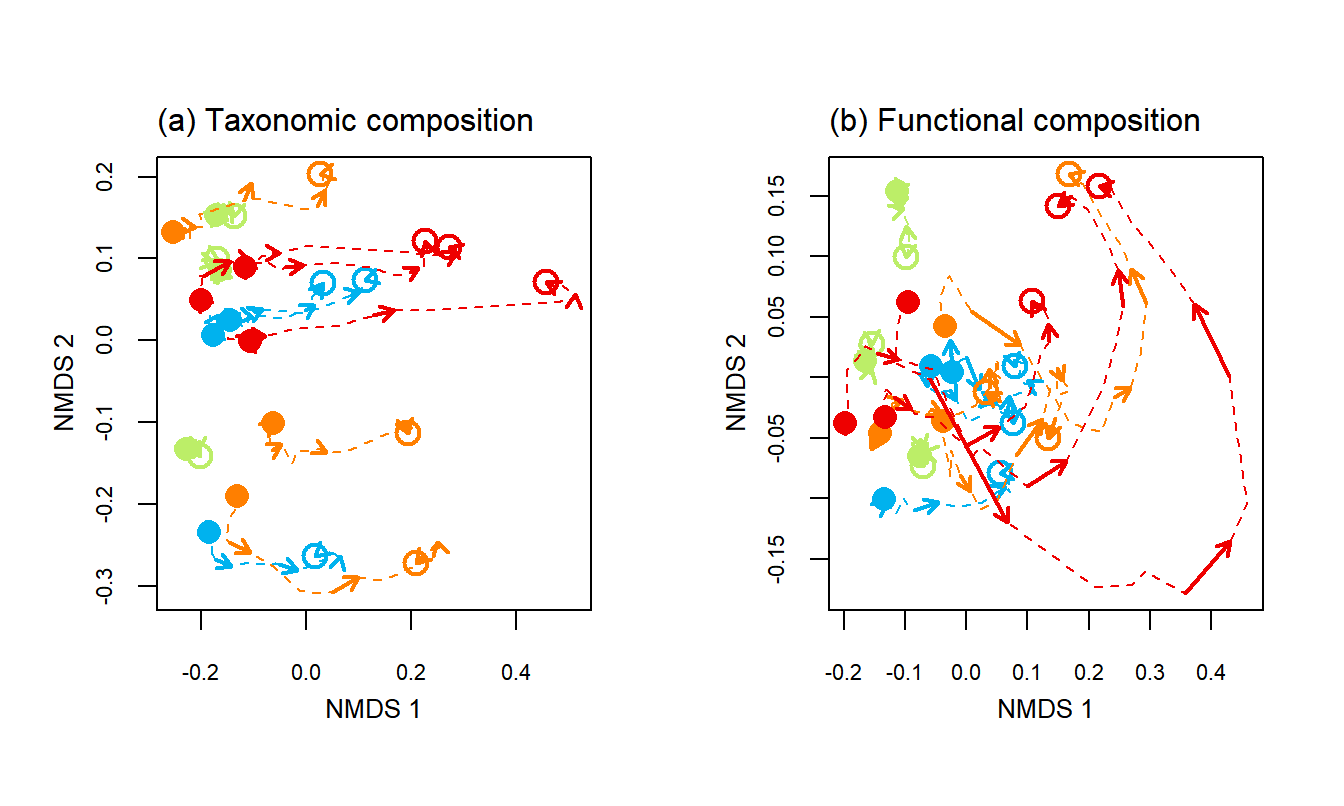
\includegraphics[width=1\linewidth]{WholePlotTrajectories_files/figure-latex/Fig1-1} 

}

\caption{Trajectories of the plots in terms of **(a)** flora composition and **(b)** functional composition regarding the 6 leaf and stem functional traits,the maximum allometric height and seed mass class in the two-dimensional space from the NMDS performed for the 30 years after disturbance. Distance matrix for NMDS were computed from the Bray-curtis dissimilarity between successive inventories. Line colors represent the disturbance treatment (green for control, blue for T1,orange for T2 and red for T3).}\label{fig:Fig1}
\end{figure*}

\begin{figure}

{\centering 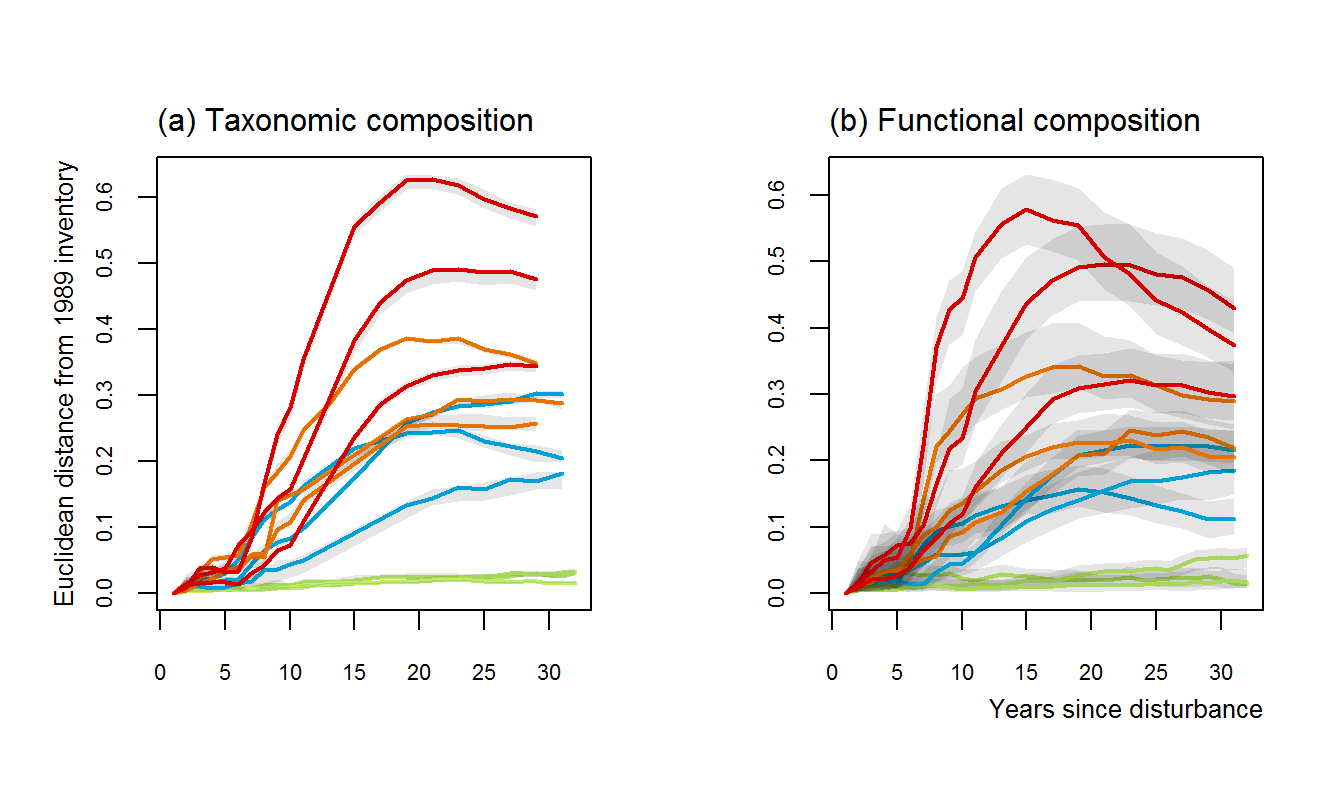
\includegraphics[width=1\linewidth]{WholePlotTrajectories_files/figure-latex/Fig2-1} 

}

\caption{Trajectories of the distance to initial condition of the 30 sampled years in the two-dimensional space from the NMDS of **(a)** taxonomic composition at genus level and **(b)** functional composition. Distance are abundance-based Bary-Curtis metric. Line colors represent the disturbance treatment (green for control, blue for T1,orange for T2 and red for T3). The 0.025 and 0.975 percentile correspond to the variance observed for 50 iteration of the taxonomic uncertainty propagation and functional trait filling processes. }\label{fig:Fig2}
\end{figure}

\subsubsection{Traits community weighted
means}\label{traits-community-weighted-means}

For all plots the trajectories of the community weighted means (CWM)
were drawn for the 8 functional and life history traits (Leaf thickness,
chlorophyll content, toughness and specific area,wood specific gravity
and barck thickness and seed mass and maximum adult height) (Figure
\ref{fig:Fig3}).

\begin{quote}
To compensate the intrinsinc difference among plots the trajectories
drawn correspond to the difference in value between the reference
inventory in \textgreater{}1984 (5 year after disturbance) and the
successive years inventoried.
\end{quote}

Except for leaf cholorphyll content, which displayed higher difference
between plots than among treatments which may be due to the completeness
of dataset, all CWM trajectories corresponded to significant changes
after disturbance. All functional traits and seed mass proportions
displayed a unimodal trajectories but with different times at maximum
and different values 30 years after disturbance. The weighted means of
communities specific maximum height at adult stage (\emph{Hmax}), leaf
toughness (\emph{L\_toughness}) and wood specific gravity (\emph{WD})
remained significantly lower than their initial value and than these of
the control plots (Figure \ref{fig:Fig3}). The weighted means of bark
thickness (\emph{Bark\_thick}) similarly remained substantilly higher
than initially for all disturbed plots while the specfic leaf area
(\emph{SLA}) had almost recovered its initial value and this of the
undisturbed plots at the end of the experiment.

\begin{figure*}

{\centering 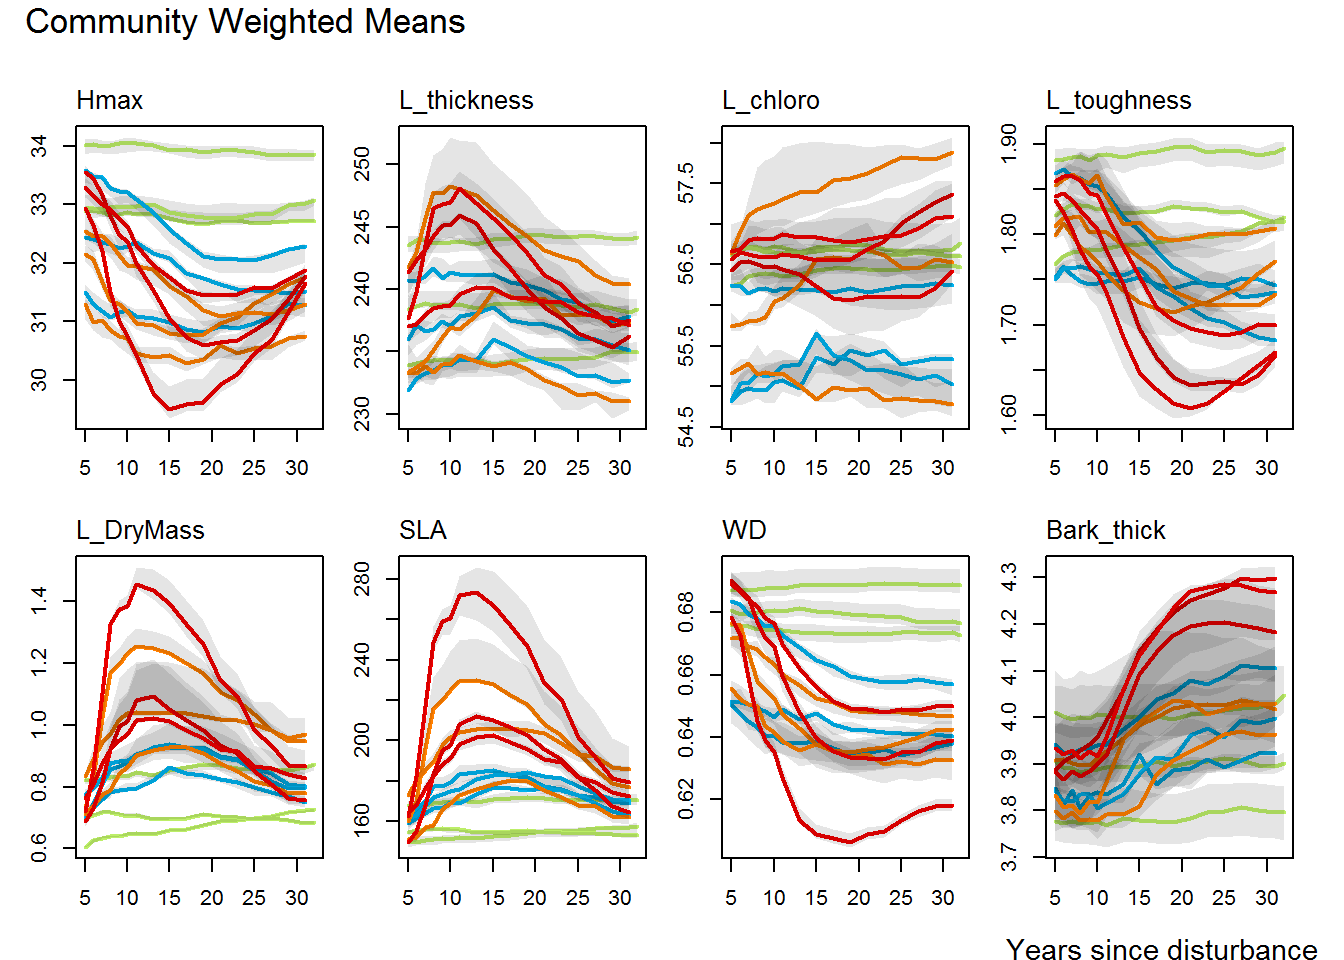
\includegraphics[width=1\linewidth]{WholePlotTrajectories_files/figure-latex/Fig3-1} 

}

\caption{Trajectories of the communities weighted means (CWM) over 30 years after disturbance of 4 leaf traits (Leaf thickness, *L_thickness*, chlorophyll content, *L_chloro*, toughness, *L_toughness* and specific area, *SLA*), 2 stem traits (wood specific gravity, *WD*, and bark thickness, *Bark-thick*) and one life trait (Specific maximum height at adult stage,*Hmax*). Trajectories correspond to the median (solid line) and 0.025 and 0.975 percentile (gray envelope) observed after 50 iteration of the taxonomic uncertainty propagation and the missing trait value filling processes. Initial treatments are represented by solid lines colorswith green for control, blue for T1,orange for T2 and red for T3.}\label{fig:Fig3}
\end{figure*}

\begin{figure*}

{\centering 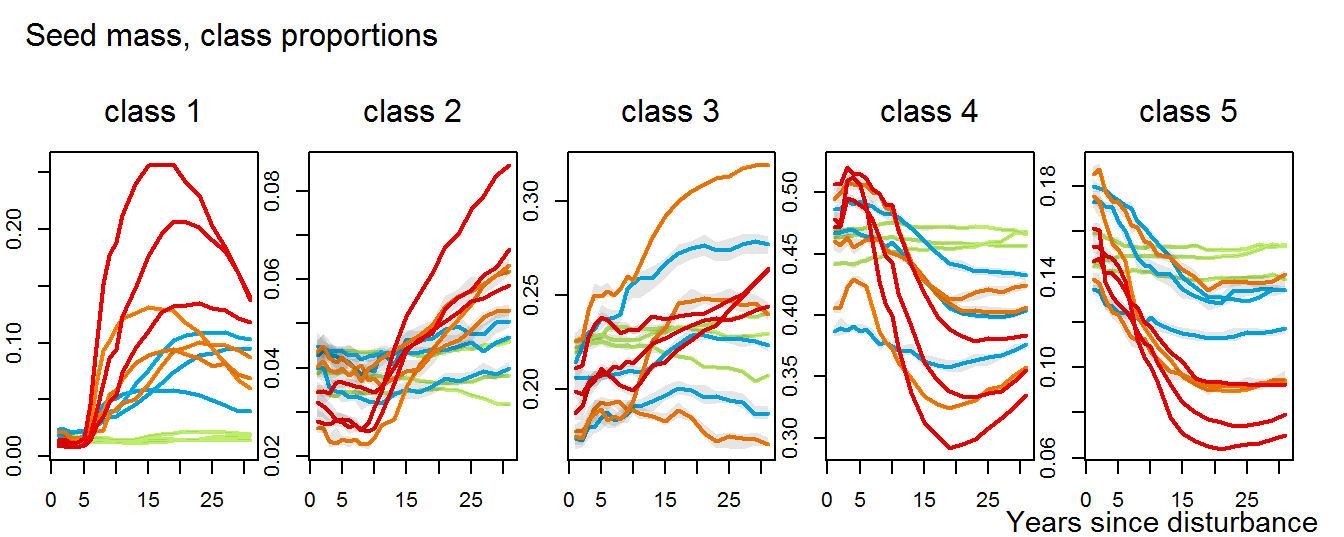
\includegraphics[width=1\linewidth]{WholePlotTrajectories_files/figure-latex/Fig4-1} 

}

\caption{Trajectories of seed mass classes proportions over 30 years after disturbance, corresponding to the median (solid line) and 0.025 and 0.975 percentile (gray envelope) observed after 50 iteration of the taxonomic uncertainty propagation. No gap filling process was applied in this case. Initial treatments are represented by solid lines colorswith green for control, blue for T1,orange for T2 and red for T3.}\label{fig:Fig4}
\end{figure*}

\subsection{Disturbance impact on
diversity}\label{disturbance-impact-on-diversity}

\subsubsection{Taxonomic diversity}\label{taxonomic-diversity}

Trajectories of Richness, Shannon and Simpson taxonomic diversity were
examined in relation to the 1989 inventories (5 years after disturbance)
(Figure \ref{fig:Fig5}). \emph{For the three indices the OLS regression
confirmed the time-dependency of the diversity variations
(P\textless{}0.01) and a covariance analysis confirmed the significant
effect of the disturbance treatment (P\textless{}0.01).}

\begin{figure*}

{\centering 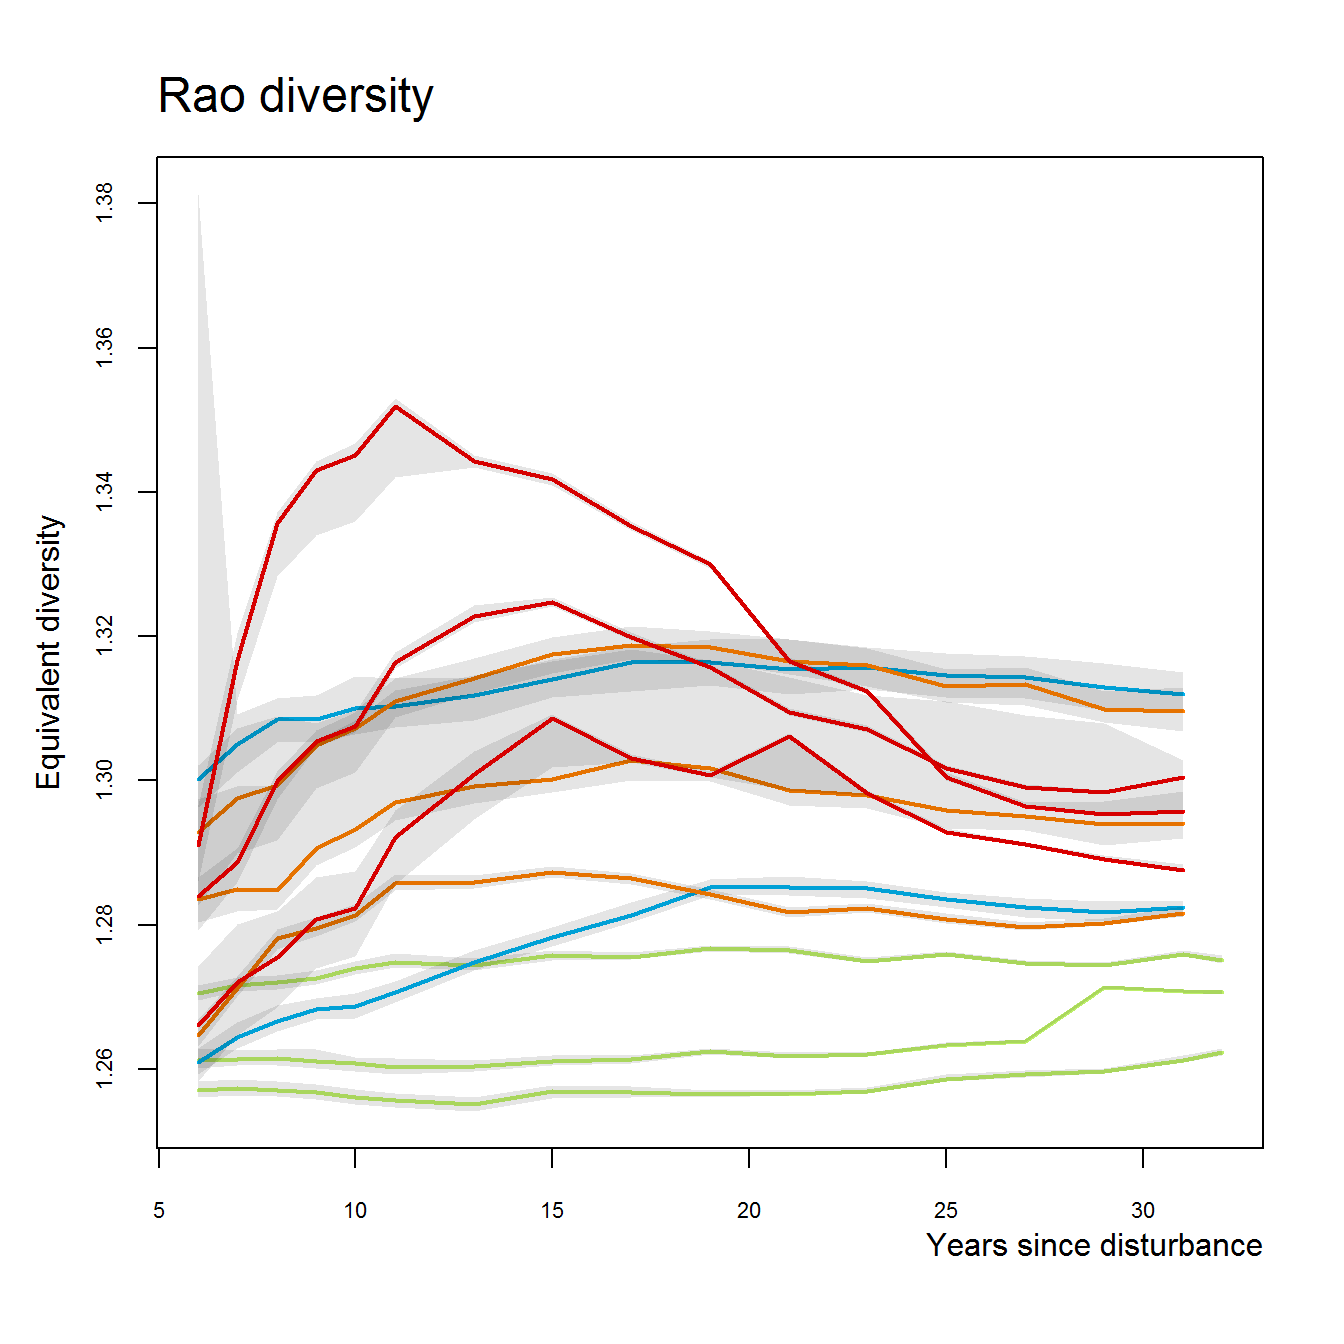
\includegraphics[width=1\linewidth]{WholePlotTrajectories_files/figure-latex/Fig5-1} 

}

\caption{Trajectories of the difference to reference inventory over 30 years after disturbance of plots communities **(a)** Richness, **(b)** Shannon and **(c)** Simpson diversities. Trajectories correspond to the median (solid line) and 0.025 and 0.975 percentile (gray envelope) observed after 50 iteration of the taxonomic uncertainty propagation. Initial treatments are represented by solid lines colorswith green for control, blue for T1,orange for T2 and red for T3.}\label{fig:Fig5}
\end{figure*}

While for undisturbed plots the Richness, Shannon and Simpson diversity
remained comparable to the values in 1989, the trajectories of all
disturbed plots showed significant increase positively correlated with
the disturbance intensity (Figure \ref{fig:Fig5}). The Richness was less
affected by the initial disturbance except for the higher intensity (T3
plots) (Figure \ref{fig:Fig5}). The Shannon and Simpson diversities
however first significantly increased, illustrating an increasing
evenness, before reaching a maximum around 15 years after disturbance
for all plots except one from T1 treatment and one from T2 treatment
(Figure \ref{fig:Fig5}).

\subsubsection{Functional diversity}\label{functional-diversity}

For all undisturbed plots the Rao diversity remained comparable to the
values in 1989, the trajectories of all disturbed plots showed
significant increase positively correlated with the disturbance
intensity (Figure \ref{fig:Fig6}). Although a first increase of plots
functional diversity that was all the more important than initial
disturbance was intense, 30 after disturbance the diversity was similar
among disturbed plots and significantly higher than this of control
plots. \emph{The OLS regression confirmed the time-dependency of the
diversity variations (P\textless{}0.01) and the covariance analysis
confirmed the significant effect of the disturbance treatment
(P\textless{}0.01)}.

\begin{figure}

{\centering 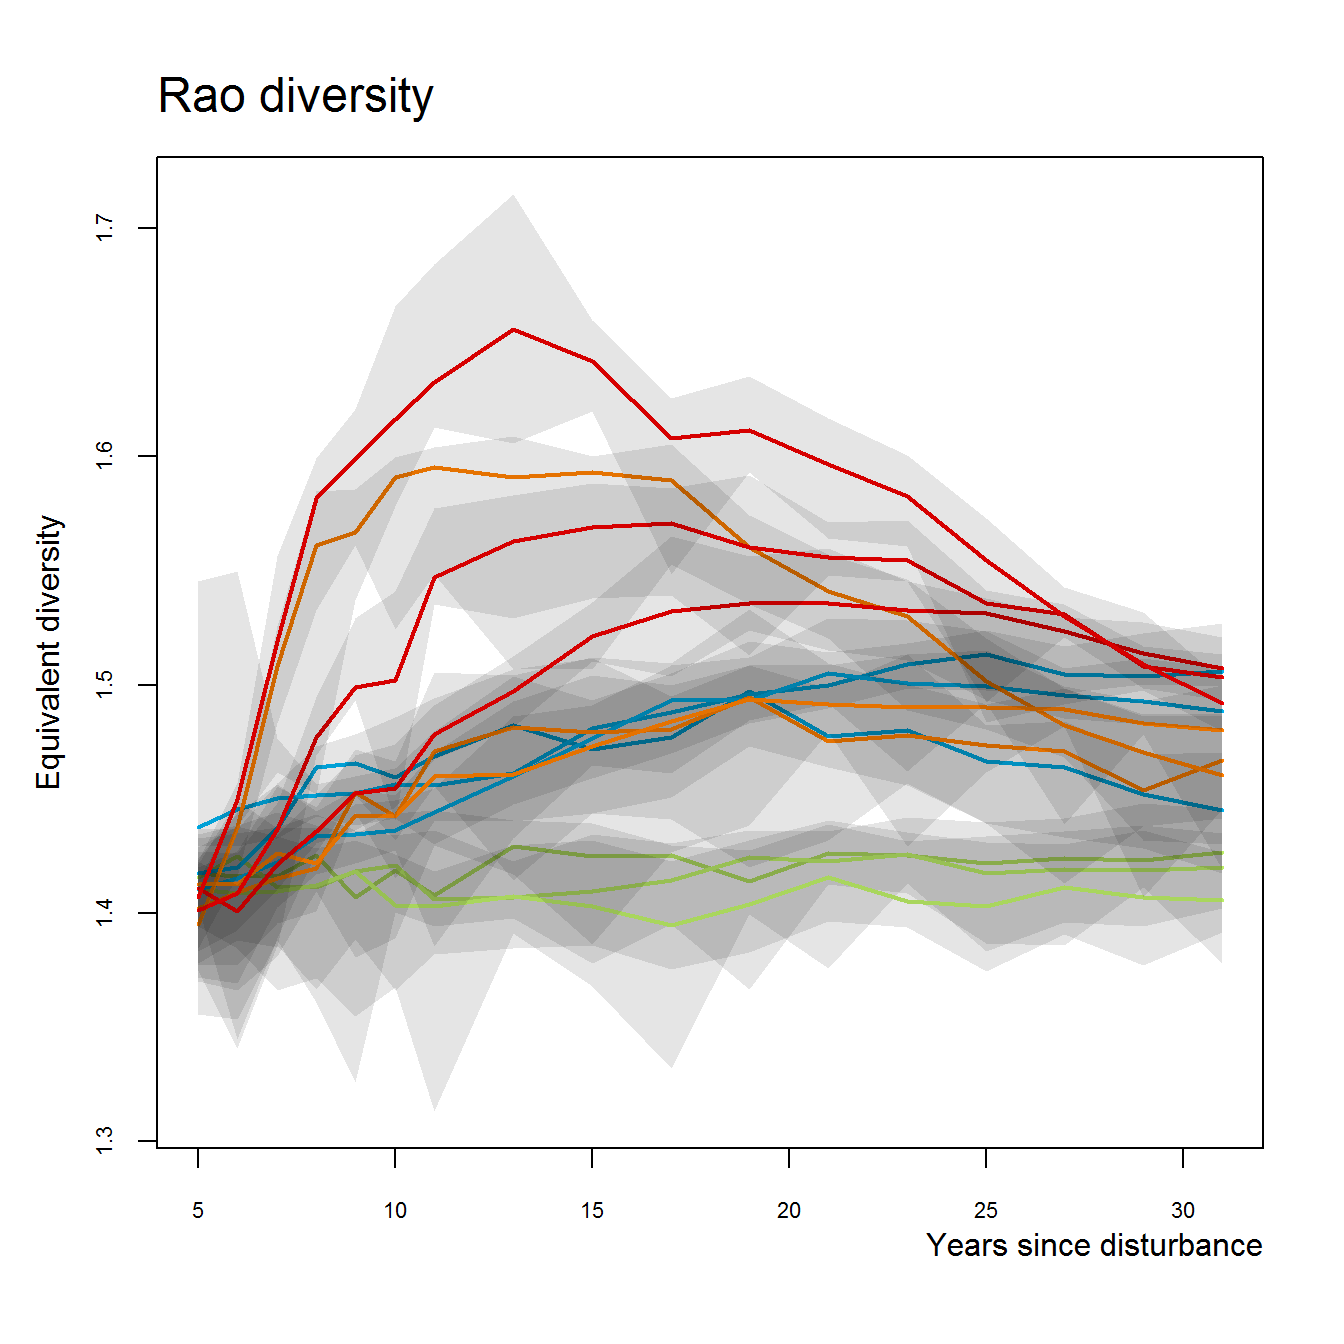
\includegraphics{WholePlotTrajectories_files/figure-latex/Fig6-1} 

}

\caption{Trajectories of the Rao functional diversity over 30 years after disturbance. Trajectories correspond to the median (solid line) and 0.025 and 0.975 percentile (gray envelope) observed after 50 iteration of the taxonomic uncertainty propagation. Initial treatments are represented by solid lines colorswith green for control, blue for T1,orange for T2 and red for T3.and the missing trait value filling processes.}\label{fig:Fig6}
\end{figure}

\section{Discussion}\label{discussion}

Our study showed the significant impact of disturbance on tropical
forests communities. The subsequent diversity trajectories confirmed the
intermediate disturbance hypothesis debated for tropical forests through
their correlation with disturbance intensity. Besides it revealed the
contrasting response of taxonomic and functional characteristics,
specifically the decoupling between communities taxonomic evenness and
their functional diversity and dominant functional traits values. The
long-term disturbance trajectories observed highlighted the unachieved
but consistent recovery of communities assembly for the lowest
disturbance intensity but questioned it after higher disturbance.

In line with the ``vegetation quantity effect'' suggesting that
communities functional characteristics depends on dominant species
rather that subtle changes in biodiversity \citep{Grime1998}. This would
result in a faster recovery of ecosystem processes rates than
composition and diversity as demonstrated for grasslands
\citep{Tilman1997, Mouillot2011} and more recently for tropical forests
\citep{Lohbeck2015, Guariguata2001}. This highlighted the functional
overlap between species in tropical forests, typical of their huge
biodiversity, and intricately questioned the different facets of
communities resilience. Ecosystem processes grasped through the set of
functional traits retained here however do not assess communities
resilience and future dynamics.

In line with the assumtions of the IDH the observed diversity
trajectories confirmed the increase of communities evenness and
functional richness after disturbance.
\textless{}\textless{}\textless{}\textless{}\textless{}\textless{}\textless{}
HEAD The consistency of the IDH has been debated for the higly diverse
tropical forests, some observing the importance of environmental filters
to shape communities assembly and others arguing for a genuine
stochastic recovery. Consistently to the trajectories drawn here, a
previous study of the same experiment revealed the directional changes
in communities composition reflecting environmental filtering after
disturbance. Disturbance regimes brought a unimodal response depending
on disturbance intensity as suggested by the outcome of 10 years and 20
years post-disturbance
analysis\citep{Hubbell1999, Molino2001, Baraloto2012a}. As observed
after logging in a Boranean rainforest \citep{Cannon1998} or after
cyclones in the Solomon islands \citep{Burslem2000}, communities
diversity showed a unimodal response to disturbance and a maintenance of
diversity levels, except for one of the intensively disturbed community
which evenness was still increasing \ref{fig:Fig5}. Despite the recovery
of communities diversity, though, taxonomic composition was clearly
altered \ref{fig:Fig3} implying a long-term, if not permenant,
composition change after disturbance as observed in East African
tropical forests \citep{Bonnell2011}.

Regarding the functional trajectories and dominant trait values of
disturbed communities (Figure \ref{fig:Fig3}), disturbance appeared to
favor acquisitive strategies, \emph{i.e} species with high SLA, low wood
density, small seeds, etc \citep{Westoby1998, Wright2004, Reich2014}.
The comparison of observed trajectories to a null model with random
traits set shuffling showed an oriented functional shift after
disturbance which suggest additional biotic and abiotic filters for the
10 to 15 years after disturbance. This means a shift from exclusive
competition favoring competitive species before disturbance to
environmental filtering selecting acquisitive and disturbance resistant
species. In particular, the evolution seed mass classes proportions
(Figure \ref{fig:Fig4}) revealed a clear increase in small seeded,
therefore large dispersive, species
\citep{TerSteege2001, Flores2006, Haddad2008}.

The diversity and composition functional trajectories showed a
decoupling between functional and taxonomic after the most intense
disturbance (treatments T2 and T3). Plots functional characteristic
returned to their initial values, similar to those of control plots,
faster than their taxonomic counterparts (Figures \ref{fig:Fig2} to
\ref{fig:Fig4}). As functional traits are the most direct link between
biodiversity and ecosystem functioning \citep{Diaz2005} the recovery of
communities functional characteristics would go along the recovery of
ecosystems processes although taxonomic composition remain altered
\citep{Guariguata2001}. Such decoupling suggested the consistency of
functional overlap and maybe functional versatility, implying a variety
of functioning from the same characteristic, in the pre-disturbance
condition. Functional overlap has been observed in highly diverse
ecosystems \citep{Bellwood2006} and suggested as one mechanisms for high
diversity maintenance. Knowing the decoupling between taxonomic and
functional trajectories, this functional overlap may not be recovering
after disturbance and therefore radically modify communities resilience
and resistance \citep{Trenbath1999, Elmqvist2003, Diaz2005}. Given the
impaired functional overlap, the persitant compositional changes
regarding disturbance resistant species \citep{Haddad2008} and probably
lianas or epiphytes \citep{Martin2013}, and the modification of
environmental conditions like soils nutrient cycling and compaction
\citep{Olander2005} the entirety of communities recovery after intense
disturbance is deeply questioned \citep{Chazdon2003a}. New conditions
would not only be longer lasting but self-maintained as tied to
disturbance regime \citep{Burslem2000}. Although communities recovered
the core of their initial functioning, composition seemed permanently
altered after intense disturbance. Specificaly, this would impair
species contingent to undisturbed forests, threatening their
maintenance, and run the risk to loose cornerstone species and trigger
unexpected ecological consequences
\citep{Jones1994, Diaz2005, Gardner2007}.

To confirm this long-term communities changes and highlight the
ecological rules shaping communities assembly, we suggest a focus on
recruitment dynamics, that would follow the diversity and functional
characteristic of recruited communities and, by extension, of the forest
to be.

\begin{quote}
Important differences among plots of same treatments: possible impact of
initial diversity composition, local abiotic parameters (topography,
soils, surrounding stands). Impacts depend on the disturbance intensity,
but further parameters may be involved.
\end{quote}

%----------------------------------------------------------------------------------------
%	REFERENCE LIST
%----------------------------------------------------------------------------------------

\bibliographystyle{mee}
\bibliography{references.bib}

%----------------------------------------------------------------------------------------

\end{document}
